\documentclass[11pt, oneside]{article}   	% use "amsart" instead of "article" for AMSLaTeX format
\usepackage{geometry}                		% See geometry.pdf to learn the layout options. There are lots.
\geometry{letterpaper}                   		% ... or a4paper or a5paper or ... 
%\geometry{landscape}                		% Activate for for rotated page geometry
%\usepackage[parfill]{parskip}    		% Activate to begin paragraphs with an empty line rather than an indent
\usepackage{graphicx}				% Use pdf, png, jpg, or eps� with pdflatex; use eps in DVI mode
								% TeX will automatically convert eps --> pdf in pdflatex		
\usepackage{amssymb}
\usepackage{amsmath}

\title{Auroux 22:  Green's Theorem}
%\author{The Author}
\date{}							% Activate to display a given date or no date

\graphicspath{{/Users/telliott_admin/Dropbox/Tex/png/}}
\begin{document}

\maketitle
%\section{}
% \subsection*{R code}
% \begin{lstlisting}  \end{lstlisting}
% \begin{center} 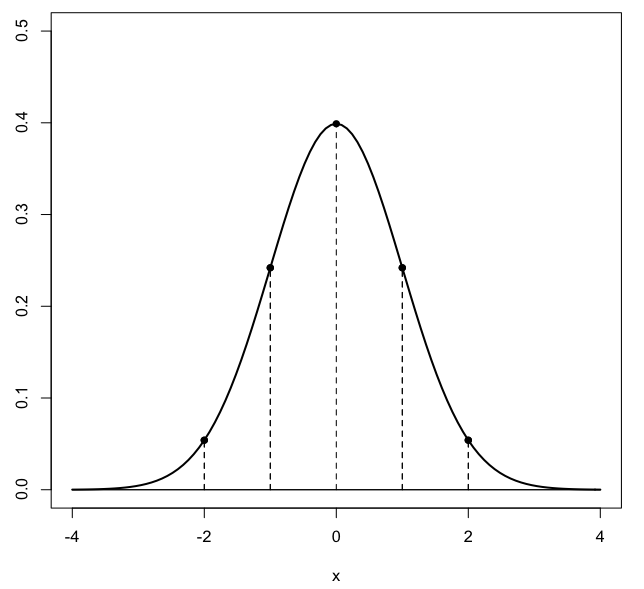
\includegraphics [scale=0.4] {gauss3.png} \end{center}
% \begin{bmatrix} a  &  b \\ c  &  d \end{bmatrix}
% \bigg |_

\large
\[ curl(F) = N_x - M_y \] for $F=\ <M,N>$.  It measures how far the field is from being conservative.  Green's Theorem is
\[ \oint_C \mathbf{F} \cdot \mathbf{dr} = \int \int_R curl(\mathbf{F}) \ dA \]
\[ \oint_C M \ dx + N \ dy  = \int \int_R (N_x - M_y) \ dA \]
where $\oint$ is an integral over a \emph{closed path}, traveling in a ccw direction.  The left-hand side "lives on the curve," whereas the right-hand side "lives over the whole region."

He gives an example where this is very useful.  Suppose
\[ M = ye^{-x}, \ \ N=\frac{1}{2}x^2 - e^{-x} \]
and our curve is a shifted unit circle, centered at $(2,0)$, so $x=2 + cos\theta$ and $y=sin\theta$.  This is trouble to parametrize, because of $e^{-x}$.  Instead do
\[ \int \int_R (N_x - M_y) dA \]
\[ M = ye^{-x}, \ \ M_y = e^{-x} \]
\[ N=\frac{1}{2}x^2 - e^{-x}, \ \ N_x = x + e^{-x} \]
\[ \int \int_R x dA \]
From lecture 21, we had $\bar{x} = (1/Area) \int \int x dA $
\[ \int \int_R x \ dA = Area(R) \ \bar{x} = \pi \ 2 \]
Alternatively, we could calculate this directly
\[ x = 2 + cos\theta, \ \ dx = -2 sin\theta \ d\theta \]
\[ y = sin \theta, \ \ dy = cos\theta d\theta \]
\[ \int \int_R x \ dA =  \int_{\theta=0}^{2\pi} \int_{r=0}^{r=1} (2 + cos\theta) \ r \ dr \ d\theta \]
inner
\[ (2 + cos\theta)\frac{r^2}{2} \ \bigg |_0^1 = 1 + \frac{1}{2}cos\theta \]
outer
\[ \int_{\theta=0}^{2\pi} (1 + \frac{1}{2}cos\theta) \ d\theta = (\theta + \frac{1}{2}sin \theta) \ \bigg |_0^{2\pi} =   2\pi \]
\subsection*{Derivation}
\vspace {2 mm}

Part 1.  We will show that
\[ \oint_C M dx = \int \int_R -M_y \ dA \]
we will do the special case where N = 0, there is only an x-component in the vector field.  but by symmetry 
\[ \oint_C N dy = \int \int_R N_x \ dA \]
and the sum is equivalent to the theorem.
\vspace{2 mm}

Part 2.  Any complex curve (with some exceptions) can be decomposed into a set of regions, we do the integrals for each one, and the boundary curves between regions cancel.
\begin{center} 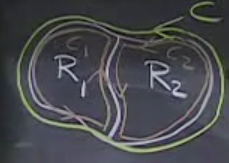
\includegraphics [scale=0.4] {regions.png} \end{center}

\vspace{2 mm}

Part 3. To prove:
\[ \oint_C M dx = \int \int_R -M_y \ dA \]
For a vertically simple region, we have a total of four curves going around
\begin{center} 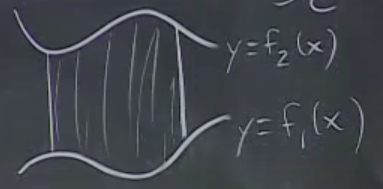
\includegraphics [scale=0.4] {Auroux22b.png} \end{center}

but two of them are vertical and have $dx=0$, the other two are
\[ \oint_C M \ dx = \oint_{C1} M \ dx + \oint_{C2} M \ dx =\int_a^b M(x, f_1(x)) \ dx - \int_a^b M(x,f_2(x)) \ dx \]
where $f_1$ is the lower curve and $f_2$ the upper one.  At each point along the curve, we have $y=f(x)$, so we can evaluate what $M(x,y)$ is at that point and then integrate with respect to $x$.  Notice that we have switched the bounds on the second integral, and added a minus sign.

Leaving that aside, now look at the right-hand side in the theorem, the integral over the region 
\[ \int \int_R -M_y \ dA = \int \int_R -M_y \ dy \ dx = - \int \int_R M_y \ dy \ dx \]
\[ M_y = \frac{\partial M}{\partial y} \]
\[ - \int_{x=a}^{x=b} \int_{f_1(x)}^{f_2(x)} \frac{\partial M}{\partial y} \ dy \ dx \]
but
\[ \frac{\partial M}{\partial y} \ dy = M \]
so (remembering the minus sign) the inner integral is just
\[ \int_{f_1(x)}^{f_2(x)} M dy = M(x, f_2(x)) - M(x, f_1(x)) \]
and the outer integral is 
\[ - \int_a^b \ [ \ M(x, f_2(x)) - M(x, f_1(x)) \ ] \ dx \]
but that is the same as what we had above (taking account of the signs).


\end{document}  